% This is part of Un soupçon de mathématique sans être agressif pour autant
% Copyright (c) 2015
%   Laurent Claessens
% See the file fdl-1.3.txt for copying conditions.



Ce chapitre va être décliné en activités mentales et exercices de début de cours. Du coup il n'y a pas de fiche d'exercices, mais tout est ici.


%+++++++++++++++++++++++++++++++++++++++++++++++++++++++++++++++++++++++++++++++++++++++++++++++++++++++++++++++++++++++++++ 
\section{Exercices de début de cours}
%+++++++++++++++++++++++++++++++++++++++++++++++++++++++++++++++++++++++++++++++++++++++++++++++++++++++++++++++++++++++++++

\let\oldcite\cite
\renewcommand{\cite}[1]{}

\newpage

\vfill
\Exo{2smath-0238}
\vfill
\newpage
\vfill
\Exo{2smath-0237}
\newpage
\Exo{2smath-0239}
\vfill
\newpage
\Exo{2smath-0240}
\vfill
\newpage
\Exo{2smath-0241}
\vfill
\newpage
\Exo{2smath-0242}
\vfill
\newpage
\Exo{2smath-0243}
\vfill

\let\cite\oldcite
\newpage

Note pour l'exercice \ref{exo2smath-0241} : le décalage d'horaire entre Paris et Tokyo est de \( 8h\). Carte à projeter éventuellement :

\begin{center}
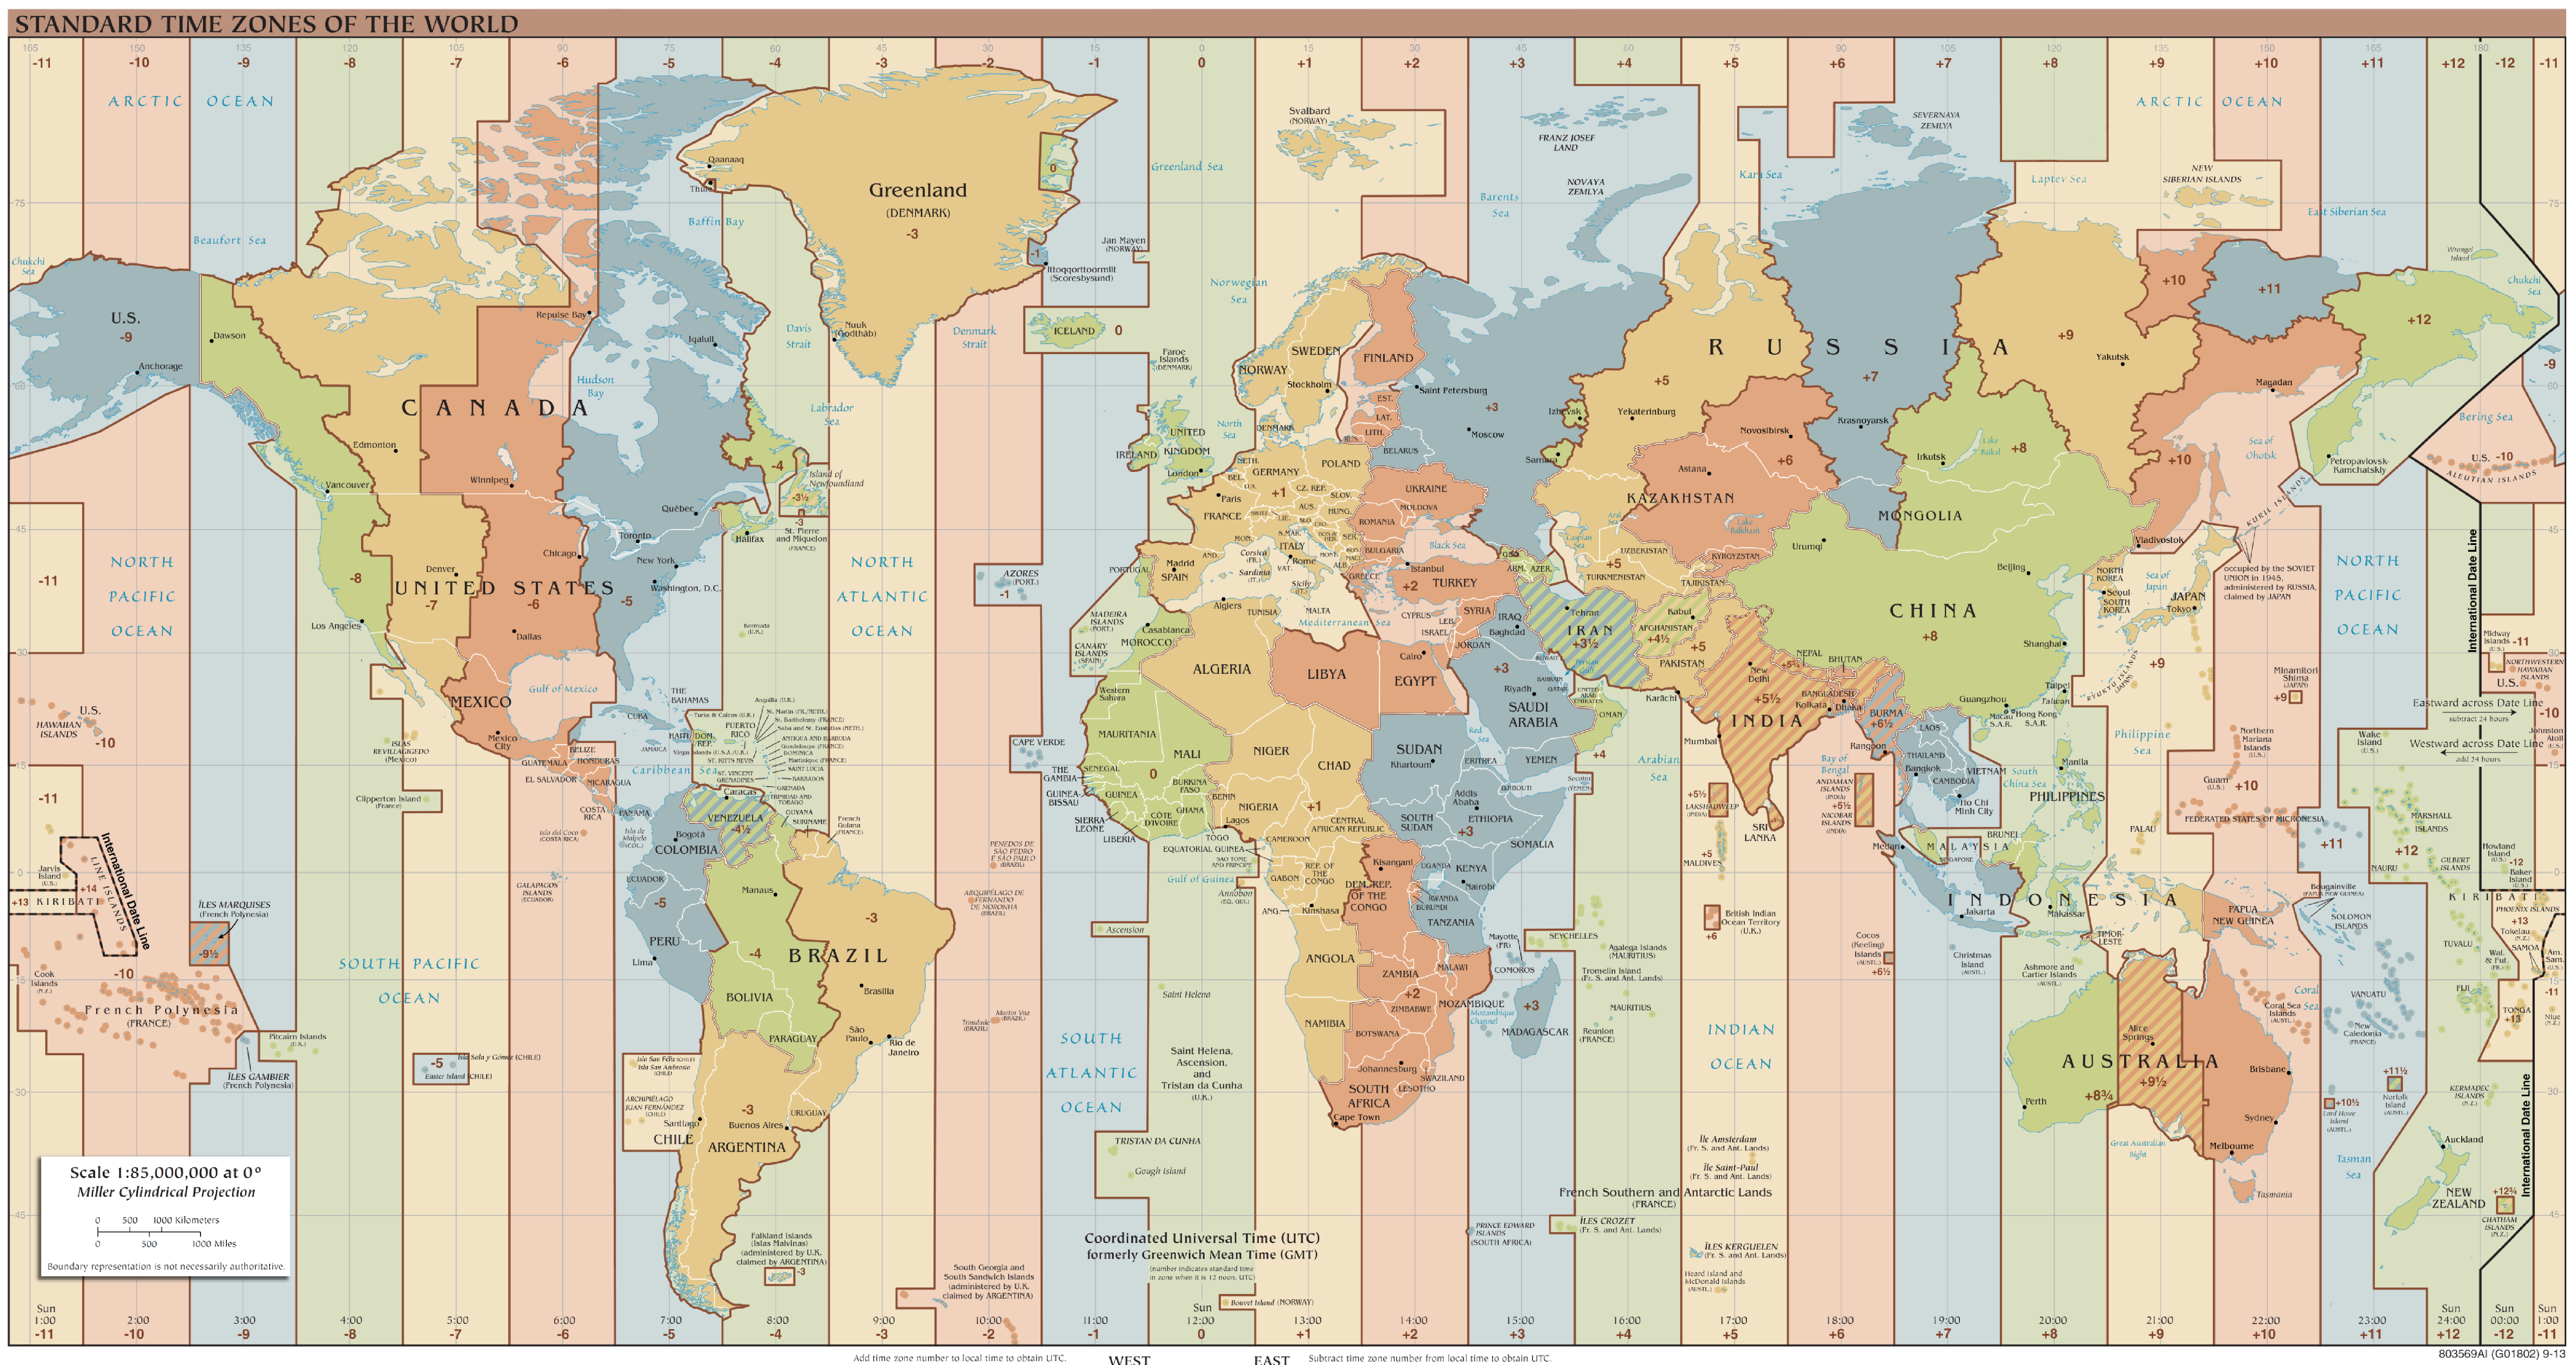
\includegraphics[width=\linewidth]{TimeZones.pdf}
\end{center}

\href{ http://creativecommons.org/licenses/by-sa/3.0/deed.fr }{Creative Commons paternité – partage à l'identique 3.0 (non transposée).)}

